
\documentclass[11pt]{beamer}
\usetheme{Frankfurt}
\usecolortheme{seahorse}
\usepackage{multirow}
\usepackage{pifont}
\usepackage{bm}
\usepackage{caption}
%\usepackage{subcaption}
\usepackage{url}


\setbeamertemplate{footline}[frame number]
\setbeamertemplate{itemize items}[triangle]
\setbeamertemplate{frametitle}[default][center]




% Symbols
\newcommand{\ra}{\rightarrow}
\newcommand{\ov}{\overline}
\newcommand{\ur}{\underline}
\newcommand{\pr}{\prime}
\newcommand{\tbf}{\textbf}
\newcommand{\omg}{\Omega}
\newcommand{\mc}{\mathcal}
\newcommand{\lt}{\left}
\newcommand{\rt}{\right}
\newcommand{\mb}{\mathbb}
\newcommand{\imp}{\implies}
\newcommand{\dimp}{\Leftrightarrow}
\newcommand{\wh}{\widehat}
\newcommand{\dg}{\mc{D}}


% Sets
\newcommand{\realset}{\mb{R}}
\newcommand{\comprealset}{\mb{\ov{R}}}
\newcommand{\pint}{\mb{Z}_{> 0}}
\newcommand{\nzrl}{\mb{R}_{\geq 0}}
\newcommand{\prl}{\mb{R}_{>0}}
\newcommand{\rl}{\mb{R}}
\newcommand{\fin}{\forall i\in\{1,...,n\}}
\newcommand{\tup}[1]{\{1,...,#1\}}
\newcommand{\seq}[2]{_{#1=1}^#2}
\newcommand{\mCnn}{\mb{M}_{n\times n}(\mb{C})}
\newcommand{\mCmm}{\mb{M}_{m\times m}(\mb{C})}
\newcommand{\mCpn}{\mb{M}_{p\times n}(\mb{C})}
\newcommand{\mCnm}{\mb{M}_{n\times m}(\mb{C})}
\newcommand{\mRnn}{\mb{M}_{n\times n}(\mb{R})}
\newcommand{\mRpn}{\mb{M}_{p\times n}(\mb{R})}
\newcommand{\mRnm}{\mb{M}_{n\times m}(\mb{R})}
\newcommand{\mRno}{{{\mb{R}}}^n_{\geq 0}}
\newcommand{\mRmo}{{{\mb{R}}}^m_{\geq 0}}
\newcommand{\mRo}{\mb{R}_{\geq 0}}
\newcommand{\mRn}{{\mb{R}}^n}
\newcommand{\mRm}{{\mb{R}}^m}
\newcommand{\mCn}{\mb{C}^n}
\newcommand{\mCm}{\mb{C}^m}
\newcommand{\inv}{\mb{GL}_n(\mb{R})}
\newcommand{\id}[1]{\mb{I}_{#1\times #1}}
\newcommand{\mat}[3]{\mb{M}_{#1\times #2}(\mb{#3})}


% matrix operations
\newcommand{\ColumnJoin}[2]{\left[\begin{array}{l}{#1}\\{#2} \end{array}\right]}
\newcommand{\minaffine}[2]{\Lambda^{\min}\lt(#1,#2\rt)}
\newcommand{\maxaffine}[2]{\Lambda^{\max}\lt(#1,#2\rt)}

% local macros
\DeclareMathOperator{\real}{\operatorname{Re}}
\newcommand{\CZ}{\lt(V,c,s\rt)}
\newcommand{\GCZ}{\gcz{V}{c}{s}{W}{l}{u}}
\newcommand{\cz}[3]{\mc{C}\lt(#1,#2,#3\rt)}
\newcommand{\CZO}{\lt(V,0,s\rt)}
\newcommand{\czo}[2]{\mc{Z}\lt(#1,0,#2\rt)}
\newcommand{\trj}[2]{{\bf #1}(#2)}
\newcommand{\IncTcz}[6]{\mc{T}\lt(#1,#2,#3,#4,#5,#6\rt)}
\newcommand{\IncGcz}[6]{\mc{G}\lt(#1,#2,#3,#4,#5,#6\rt)}
\newcommand{\Ptope}[3]{\mc{P}\left(#1,#2,#3\right)}
\newcommand{\gcz}[6]{\mathcal{Z}\lt(#1,#2,#3,#4,#5,#6\rt)}
\newcommand{\sptope}[3]{\mathcal{P}\lt(#1,#2,#3\rt)}
\newcommand{\system}{\mb{H}}
\newcommand{\locationset}{Q}
\newcommand{\edgeset}{E}
\newcommand{\stay}{\gamma}
\newcommand{\linearmapset}{\mc{A}}
\newcommand{\inputset}{U}
\newcommand{\initialset}{\Omega}
\newcommand{\edge}{\sigma}
\newcommand{\loc}{q}
\newcommand{\map}{\linearmapset}
\newcommand{\inp}{\inputset}
\newcommand{\ptemplate}{\mc{K}}
\newcommand{\systrj}[2]{\lt({\bf #1},{\bf #2}\rt)}
\newcommand{\wholenums}{\mb{Z}_\geq 0}
\newcommand{\preloc}[1]{#1_{1}}
\newcommand{\postloc}[1]{#1_{2}}
\newcommand{\upperedgebound}[1]{#1^+}
\newcommand{\loweredgebound}[1]{#1^-}
\newcommand{\reset}[1]{#1_r}
\newcommand{\locationtransition}[1]{R_{#1}}
\newcommand{\edgetransition}[1]{R_{#1}}
\newcommand{\staysptope}[1]{\sptope{\ptemplate\lt(#1\rt)}{\stay^-\lt(#1\rt)}{\stay^+\lt(#1\rt)}}
\newcommand{\guardsptope}[1]{\sptope{\ptemplate\lt(\preloc{#1}\rt)}{\max\lt(\loweredgebound{#1},\stay^-\lt(\preloc{#1}\rt)\rt)}{\min\lt(\upperedgebound{#1},\stay^+\lt(\preloc{#1}\rt) \rt)}}
\newcommand{\hybridset}{\Gamma}
\newcommand{\transfer}[4]{#1#4 = #2\dg\lt(#3\rt)}
\newcommand{\centertransfer}[4]{#1#4 = #3-#2}
\newcommand{\scalebound}[5]{\max_{i=1}^{#4}\lt(\lt(\sum_{j=1}^{#5}\lt|#1\rt|_j\rt)-#3_i+#2_i\rt)}
\newcommand{\pseudoinverse}[1]{#1\lt(#1#1^T\rt)^{-1}}


\title{Augmented complex zonotopes for computing invariants of affine hybrid systems}
\setbeamercolor{author}{fg=blue}
\author[shortname]{{  \bf \hspace{-1em} Arvind\ Adimoolam~\inst{1}\hspace{1em} Thao\ Dang~\inst{2}}}
\setbeamercolor{institute}{fg=blue}
\institute{{\bf 
\inst{1,2} VERIMAG/ \inst{2}CNRS}\\~Grenoble,France
\begin{figure}
\center
\hspace{2em}
\includegraphics[scale=0.2]{figures/LogoVERIMAG.png}
\end{figure}
}

\date{}

\begin{document}
\maketitle

\begin{frame}{Discrete time dynamical system}
Models \textcol{evolution of system state} at \textcol{discrete time instants} by a
possibly \textcol{non-deterministic transition function}.
\begin{block}{}
%
{
\begin{align*}
& \trj{x}{t+1}\subseteq f\lt(\trj{x}{t},\trj{u}{t}\rt)\\
& f:\reals^n\ra 2^{\reals^n}~~\text{(transition function)}\\
& \trj{x}{0}\in\init~~\text{(initial set)}\\
& \trj{u}{t}\in\inputset ~~\text{(input set).}
\end{align*}
}
%
\end{block}
%
\begin{figure}
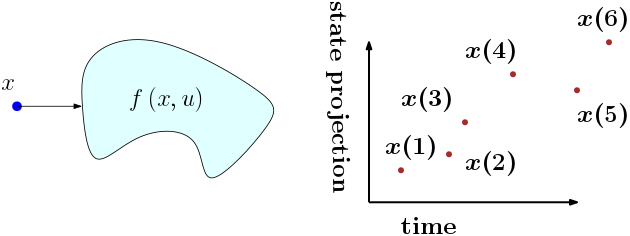
\includegraphics[scale=0.35]{figures/dynamical-system.png}
\end{figure}
%
\end{frame}

\begin{frame}{Discrete time affine hybrid system}
Let \textcol{$x\in\reals^n$ (continuous state)} and \textcol{$q\in\set{1,...,l}$ (discrete state)}.

Transition function $f$ is of the following form:
%
\begin{block}{}
%
\begin{align*}
& f(x,q)=\bigcup_{i=1}^h\lt(f_i(x),g_i(q)\rt)
\end{align*}
\vspace{-2em}
%
{\bf
\begin{align*}
 & \lt\{
\begin{array}{l}
\text{if}~~T x\leq d\\
~~~f_i(x,q) \subseteq \lt(A_ix\oplus\inputset_i\rt)\bigcap S_{g_i(q)}\\
\text{else}\\
~~~\emptyset.
\end{array}
\rt.
\end{align*}
}
%
\end{block}
%
\end{frame}

%
\begin{frame}{Reachable set}
The \textcol{reachable set} at time \textcol{$t$} is defined inductively as
%
\eqncol{
\[
\reachset{t}=\bigcup_{x\in\reachset{t-1},u\in\inputset}f\lt(x,u\rt).
\]
}
%
{Applications} of reachable set computation:
%
\begin{enumerate}
\item \textcol{Safety verification}.
\item \textcol{Stability verification}.~\cite{todo}
\end{enumerate}
%
\begin{figure}
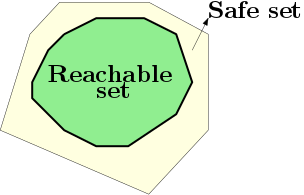
\includegraphics[scale=0.4]{figures/safety.png}
\end{figure}
%
\end{frame}
%

\begin{frame}{Set-representation for approximating reachable sets}.
\begin{itemize}
\item For a \emph{discrete time affine hybrid system}, the \emph{reachable set at a
time point} is a \eqncol{union} of number of sets \eqncol{exponential in the number of
discrete variables}.\pause
% \item \eqncol{Intractable computational complexity} of exact computation.
\item Instead, use a \textcol{set of smaller representation size} to
\textcol{over-approximate} reachable set.\pause
\end{itemize}
%
\begin{alertblock}{}
{\bf Set representation}: {\color{blue} Data structure} used to denote
a {\color{blue} geometric shape}.  Eg. {\color{purple} Polytope}: $\lt(T,d\rt): Tx\leq d$,
{\color{purple} Ellipsoid}: $\lt(P\rt): x^TPx\leq 1$.
\end{alertblock}
%
\begin{figure}
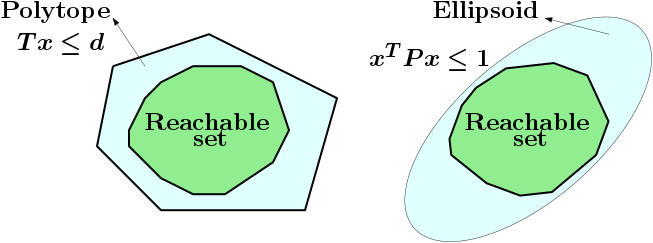
\includegraphics[scale=0.35]{figures/set-representation.png}
\end{figure}
%
\end{frame}

\begin{frame}{Bounded time reachable set approximation}
\begin{itemize}
\item Reachable set over a \textcol{finite time horizon} is
approximated as a \textcol{finite union of sets}, the \textcol{number
of sets} are equal to the \textcol{number of time points}.
%
{
\begin{align*}
& \reachset{\lt[\begin{matrix}0 & T\end{matrix}\rt]}\subseteq\bigcup_{t=1}^T\alpha(t)\\
& \reachset{t}\subseteq\alpha(t).
\end{align*}
}
%
\end{itemize}
%
\end{frame}

\begin{frame}{Unbounded time reachable set approximation}
%
\begin{block}{Positive invariant}
$P\subseteq\reals^n$ is a positive invariant if
%
$
\bm{\forall x\in P, f(x)\in P}.
$
%
\end{block}
%
\begin{itemize}
\item
{\color{blue} Positive invariance $\Rightarrow$} Proof of
{\color{blue} valid over-approximation} for \underline{unbounded
time}.
\item {$\init\in \operatorname{Positive~Invariant}$}
$\implies$ {$\operatorname{Reachable~Set}\subseteq \operatorname{Positive~Invariant}$}.
\end{itemize}
%
\begin{figure}
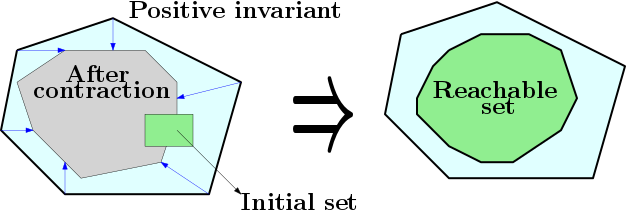
\includegraphics[scale=0.35]{figures/positive-invariant.png}
\end{figure}
%
\end{frame}

\begin{frame}{Desirable features of a good set representation}
%
\begin{enumerate}
\item \textcol{Efficient closure} under \textcol{reachable set
computations} like {\it matrix
multiplication, Minkowski sum, intersection with linear constraints}, $\Rightarrow$
 Good \textcol{approximation quality}.
%
\begin{itemize}
\item \eqncol{Polytopes} efficiently closed under \eqncol{intersection with linear
constraints}.
\item \eqncol{Ellipsoids} efficiently closed under \eqncol{matrix multiplication}.
\item \eqncol{Zonotopes} closed under \eqncol{matrix multiplication} and \eqncol{Minkowski sum}.
\end{itemize}
\pause
%
\item Existence of \textcol{efficiently computable positive invariants} in the
\textcol{linear case}.  Example: \eqncol{Ellipsoids}.
\end{enumerate}
%
\end{frame}

\begin{frame}{Simple Zonotope}
%
\begin{itemize}
\item Let {\color{purple} $\stemp\in\mat{n}{k}{\reals}$} called {\color{blue}
generator matrix} and {\color{purple} $\cen\in\reals^n$} called the
{\color{blue} center.}
%
\[
{\color{purple}
\rztope{\stemp}{\cen}=\set{\cen+\stemp\zeta:\zeta\in\reals^k,\infnorm{\zeta}\leq 1}
}
\]
\item Geometrically, {\color{blue} Minkowski sum of line segments}.
\end{itemize}
\begin{minipage}{0.65\textwidth}
\begin{figure}
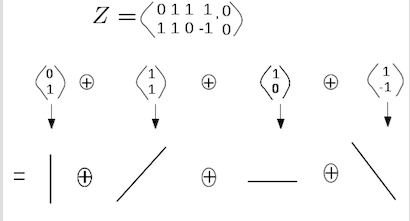
\includegraphics[trim={2mm 0 2mm 1.5cm},clip,scale=0.45]{figures/rz1.png}
\end{figure}
\end{minipage}
%
\begin{minipage}{0.25\textwidth}
\begin{figure}
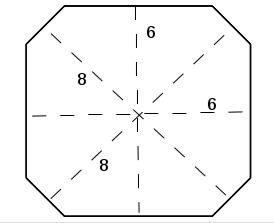
\includegraphics[trim={0 3cm 0 0},scale=0.4]{figures/rz2.png}
\end{figure}
\end{minipage}
%
{\small
\begin{thebibliography}{1}

\bibitem{girard2005reachability}
Antoine Girard.
\newblock Reachability of uncertain linear systems using zonotopes.
\newblock In {\em HSCC}, volume~5, pages 291--305. Springer, 2005.

\end{thebibliography}
}
\end{frame}

\begin{frame}{Advantage of zonotopes}
\begin{itemize}
\item Zonotopes are \textcol{efficiently closed} under \textcol{matrix
multiplication} and {Minkowski sum}.
\item Good for approximating \textcol{ bounded time reachable set}
of \textcol{uncertain linear systems} and some classes
of \textcol{affine hybrid systems}.
\end{itemize}
\pause
\eqncol{What about unbounded time, i.e., computation of positive invariant?}
\end{frame}

\begin{frame}{Disadvantage of zonotope}
%
\begin{itemize}
\item \eqncol{Existence of positive invariant zonotope} for a {\it deterministic linear
system} is \eqncol{not guaranteed}.
\end{itemize}
\pause
%
Our solution:
%
\textcol{Extend} simple zonotope to \textcol{complex domain} to
capture invariance based on \textcol{complex eigenstructure}.
\end{frame}

\begin{frame}{Complex zonotope}
%

\emph{Linear combination} of
\emph{ complex-valued eigenvectors} such that \emph{
complex combining coefficients} are  bounded in \emph{absolute
values}.

%
\begin{block}{}
Let \eqncol{$\ptemp\in\mat{n}{m}{\compnums}$} called \textcol{template},
\eqncol{$\cen\in\compnums^n$} called \textcol{center} and \eqncol{$\sfact\in\reals_{\geq 0}^m$}
called \textcol{scaling factors}.
%
{\color{black}
\[
\bm{
\tcztope{V}{c}{s}=\set{V\zeta+c:~\zeta\in\compnums^m,~\absolute{\zeta}\leq
s}
}
\]
}
\end{block}
%
\end{frame}

\begin{frame}{Geometric visualization: Complex zonotope}
\begin{itemize}
\item Represent {\color{blue} wider class of sets} than {\it real zonotopes}.
\item {\it Minkowski sum} of {\color{blue} some ellipsoids} in
addition to {\color{blue}line segments}.
\item Can represent some {\color{blue} non-polyhedral sets} in
along with {\color{blue} polytopic real zonotopes}.
\end{itemize}
%
\begin{figure}
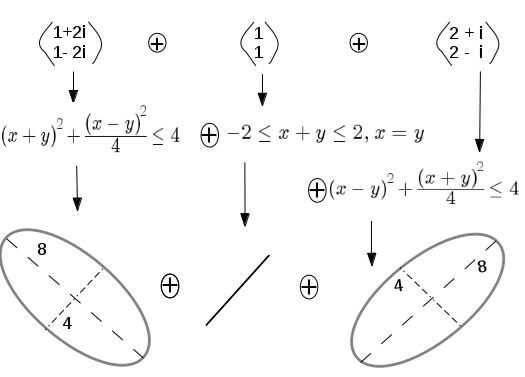
\includegraphics[scale=0.45]{figures/complex-zonotope.png}
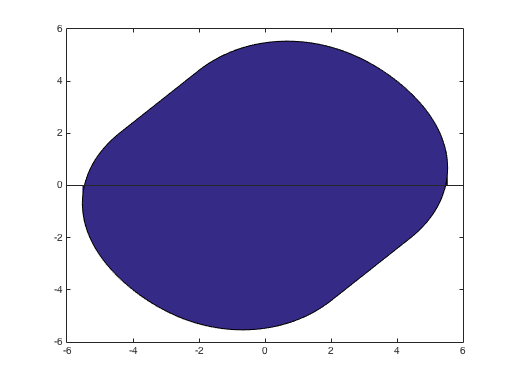
\includegraphics[scale=0.3]{figures/CZhull.png}
\end{figure}
%
\end{frame}

\begin{frame}{Advantage: Complex eigenstructure based positive invariance}
Consider {\color{blue} matrix $A\in\mat{n}{n}{R}$} with {\color{blue} eigenvectors $e_1,...,e_n$}
and {\color{blue} $\mu$: vector of eigenvalues}.
%
{\color{purple}
\begin{align*}
 A\tcztope{[e_1,...,e_n]}{0}{\sfact}   = \tcztope{[e_1,...,e_n]}{0}{\diagonal{\absolute{\mu}}\sfact}
\end{align*}
}
%
\center{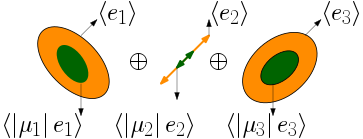
\includegraphics[scale=0.6      ]{figures/ContractionCZ.png}}
\end{frame}

\begin{frame}{A drawback of complex zonotope}
%
\begin{itemize}
\item {\it Complex zonotopes} are \eqncol{not closed} under \eqncol{intersection} with
\eqncol{ sub-level sets of linear inequalities}.
\pause
\item
Solution:
\textcol{Augmented complex zonotope}: {\it Minkowski sum} of {\it complex
zonotope} and \textcol{interval zonotope}.
\end{itemize}
%
\end{frame}

\begin{frame}{Interval zonotope}
%
\begin{itemize}
\item Let {\color{purple} $W\in\mat{n}{k}{\reals}$} called {\color{blue}
template}, {\color{purple} $l,u\in\reals^k:~l\leq u$} called
{\color{blue} upper and lower coefficient bounds}.
%
\[
{\color{purple}
\iztope{W}{l}{u}=\set{W\zeta:\zeta\in\reals^k,~l\leq \zeta\leq u}
}
\]
\item \eqncol{Geometrically} the \eqncol{same as real zonotope}, but has \textcol{different
representation} that \textcol{facilitates computing intersection} with
a \underline{class of linear inequalities}.
\end{itemize}
%
\end{frame}

\begin{frame}{Sub-parallelotope}
Equivalent to possibly \textcol{ unbounded parallelotopes}.
%
\begin{block}{Definition}
Let \eqncol{${\qtemp}\in\mat{k}{n}{\reals}$} such that
\eqncol{$\lt(\qtemp\transpose{\qtemp}\rt)$} is an \textcol{invertible square matrix}.  We
call such a matrix $\qtemp$ as a \textcol{sub-paralleotopic template}.
Let \eqncol{$\plb,\pub\in\set{\reals,-\infty,\infty}^k$} such that
\eqncol{$\plb\leq\pub$}, called \textcol{ lower and upper offsets}, respectively.
%

\[\bm{
\ptope{\qtemp}{\plb}{\pub}=\set{x\in\reals^n:~\plb\leq\qtemp x\leq\pub}.
}
\]
%
\end{block}
%
\end{frame}

\begin{frame}{Relation of Sub-parallelotope to generator representation}
Notation: $\pinv{\qtemp}=\transpose{\qtemp}\inv{\lt(\qtemp\transpose{\qtemp}\rt)}$.
%
\begin{proposition}[Relation to generator representation]
  Consider a sub-parallelotope
  \eqncol{$\ptope{\qtemp}{\plb}{\pub}$} where \eqncol{$\qtemp\in\mat{k}{n}{\reals}$}.
  Then, $\bm{\ptope{\qtemp}{\plb}{\pub}}$\vspace{-1em}
  %
  \[
   \bm{=\set{\cen+\pinv{\qtemp}\zeta:~c\in\reals^n,\zeta\in\reals^k,~\qtemp
  \cen=0,~\plb\leq
  \zeta\leq \pub
  }.
  }
  \]
  %
\end{proposition}
%
\end{frame}

\begin{frame}{Intersection: Interval Zonotope and Sub-parallelotope}

\textcol{Interval zonotopes} are \textcol{efficiently closed} under \textcol{intersection}
with \textcol{aligned} \textcol{ sub-parallelotopes}.  
%
\begin{lemma}~\label{lem:motivation}
Let \eqncol{$K\in\mat{k}{n}{R}$} be a sub-parallelotopic template.  Then
%
\[\bm{
\iztope{\pinv{\qtemp}}{\lb}{\ub} \bigcap \ptope{\qtemp}{\plb}{\pub}
= \iztope{\pinv{\qtemp}}{\lb\bigvee \plb}{\ub\bigwedge \pub}
}
\]
\end{lemma}
%
\end{frame}

\begin{frame}{A Useful Theorem about Convex Sets}
\begin{lemma}~\label{gen-int}
Let {\it $S_1\subseteq \compnums^n$} and {\it $S_2,S_3\in\reals^n$}
be {\it closed
convex sets} such that {$\intersection{S_2}{S_3}\neq \emptyset$} and
{$0\in S_1$}.
%
\begin{align}~\label{eqn:minsum-intersection}
& \bm{\intersection{\lt(S_1\oplus S_2\rt)}{S_3}\subseteq S_1\oplus\lt(\intersection{S_2}{S_3}\rt)}.
\end{align}
%
\end{lemma}
\pause
%
\begin{exampleblock}{Result}
Let $S_1=\tcztope{\ptemp}{\cen}{\sfact}: 0\in S_1$,
$S_2=\iztope{\pinv{\qtemp}}{\lb}{\ub}$,
$S_3=\ptope{\qtemp}{\plb}{\pub}$.
%
\eqncol{
\begin{align*}
& \intersection{\lt(\minsum{\tcztope{\ptemp}{\cen}{\sfact}}{\iztope{\pinv{\qtemp}}{\lb}{\ub}}\rt)}{\ptope{\qtemp}{\plb}{\pub}}\\
& \subseteq \minsum{\tcztope{\ptemp}{\cen}{\sfact}}{\lt(\intersection{\iztope{\pinv{\qtemp}}{\ptope{\qtemp}{\plb}{\pub}}}\rt)}\\
& = \minsum{\tcztope{\ptemp}{\cen}{\sfact}}{\iztope{\pinv{\qtemp}}{\join{\lb}{\plb}}{\meet{\ub}{\pub}}}.
\end{align*}
}
%
\end{exampleblock}
%
\end{frame}

\begin{frame}{Augmented complex zonotope}

\begin{block}{Definition}
Let us consider \eqncol{complex matrix $\ptemp$}, called \textcol{primary
template}, \eqncol{complex vector $\cen$}, called \textcol{primary offset}, \eqncol{real matrix
$\stemp$}, called \eqncol{secondary template} and \eqncol{real vectors
$\lb,\ub:~\lb\leq\ub$}, called \textcol{lower and upper interval bounds}.
%
\[
\bm{\acztope{\ptemp}{\cen}{\sfact}{\stemp}{\lb}{\ub}=\minsum{\tcztope{\ptemp}{\cen}{\sfact}}{\iztope{\stemp}{\lb}{\ub}}}.
\]
%
\end{block}
%
\textcol{Reason for abover representation}: If $0\in\tcztope{\ptemp}{\cen}{\sfact}$, then
%
\begin{theorem}[Intersection with Sub-parallelotope]
\vspace{-1em}
%
\begin{align*}
& \acztope{\ptemp}{\cen}{\sfact}{\pinv{\qtemp}}{\lb}{\ub}\bigcap\ptope{\qtemp}{\plb}{\pub}\\
& \subseteq \acztope{\ptemp}{\cen}{\sfact}{\pinv{\qtemp}}{\join{\lb}{\plb}}{\meet{\ub}{\pub}}.
\end{align*}
%
\end{theorem}
%
\eqncol{Over-approximation error} along any direction is proportional
to \eqncol{orientation between primary and secondary templates}.
\end{frame}






\begin{frame}{Affine over-approximation of intersection}
\begin{exampleblock}{Affine approximation of multi-variable Min and Max functions}
{\small
\begin{itemize}
\item \textcol{Min-approximation function}:
$\lt(\minaffine{u}{\wh{u}}\rt)_i = \left\{
\begin{array}{l}
\wh{u}_i~~\text{if}~\wh{u}_i<\infty\\
u_i~~\text{if}~\wh{u}_i=\infty
\end{array}
\right..$\\
\item \textcol{Max-approximation function}:
$\lt(\maxaffine{l}{\wh{l}}\rt)_i = \left\{
\begin{array}{l}
\wh{l}_i~~\text{if}~\wh{l}_i>\infty\\
l_i~~\text{if}~\wh{l}_i=-\infty
\end{array}
\right..$
\end{itemize}
}
\end{exampleblock}
\begin{block}{Corollary}~\label{thm:acz-int}
{\small Given sub-parallelotope {$\sptope{\ptemplate}{\wh{l}}{\wh{u}}$},
augmented complex zonotope {$\gcz{V}{c}{s}{\pinv{\ptemplate}}{l}{u}$}
such that {$V\conjtranspose{V}$ is non-singular, $\lt|\pinv{V}c\rt|\leq s$, $l\leq
\maxaffine{l}{\wh{l}}\leq \minaffine{u}{\wh{u}}\leq u$}:}
\vspace{-1em}
{\color{purple}
\begin{align*}
\begin{split}
&{\gcz{V}{c}{s}{\pinv{\ptemplate}}{l}{u}\bigcap\sptope{\ptemplate}{\wh{l}}{\wh{u}}}\\
& {\subseteq \gcz{V}{c}{s}{\pinv{\ptemplate}}{\maxaffine{l}{\wh{l}}}{\minaffine{u}{\wh{u}}}}
\end{split}
\end{align*}
}
\end{block}
\end{frame}


\begin{frame}{Minkowski sum and Linear Transformation}
\begin{block}{Affine function for fixed templates}
\begin{enumerate}
\item $A\gcz{V}{c}{s}{W}{l}{u} = \gcz{AV}{Ac}{s}{AW}{l}{u}$.
\item $~$\vspace{-2em}\hspace{-2em}\begin{align*}
&\gcz{V}{c}{s}{W}{l}{u}\oplus\gcz{V^\pr}{c^\pr}{s^\pr}{W^\pr}{l^\pr}{u^\pr}\\
&= \gcz{\lt[V~V^\pr\rt]}{c+c^\pr}{\ColumnJoin{s}{s^\pr}}{\lt[W~W^\pr\rt]}{\ColumnJoin{l}{l^\pr}}{\ColumnJoin{u}{u^\pr}}.
\end{align*}
\end{enumerate}
\end{block}
%
%% \begin{alertblock}{}
%% \begin{itemize}
%% \item For \eqncol{fixed primary and secondary templates} of augmented complex zonotopes, {\bf Linear transformation and Minkowski sums} of are \textcol{Affine functions of rest variables}.
%% \end{itemize}
%% \end{alertblock}
\end{frame}
%
\begin{frame}{Inclusion between Template Complex Zonotopes}
Let \textcol{$\cz{V^\pr_{n\times
    m^\pr}}{c^\pr}{s^\pr}\order \cz{V_{n\times m}}{c}{s}$} if
\eqncol{\begin{align*}~\label{eqn:tcz-inc}
\begin{split}
& \exists X\in\mat{m}{m^\pr}{\mb{C}}~\text{and}~y\in\mb{C}^{m}~\text{s.t.}\\
& \transfer{V}{V^\pr}{s^\pr}{X},~~~\centertransfer{V}{c}{c^\pr}{y},~\text{and}~
 \scalebound{X}{y}{s}{m}{m^\pr}\leq 0\\
\end{split}
\end{align*}
}
\textcol{Theorem}: \eqncol{$(\order)\implies(\subseteq)$} among \eqncol{Template Complex zonotopes}.
%
\begin{alertblock}{}
For fixed \eqncol{template}, \textcol{$\order$} defines \textcol{SOCC (convex constraints) on remaining variables}.
\end{alertblock}
\end{frame}
%
\begin{frame}{Real Inclusion between Augmented Complex Zonotopes}
\begin{block}{}
Let \textcol{$\gcz{V^\pr}{c^\pr}{s^\pr}{W^\pr}{l^\pr}{u^\pr}\order
\gcz{V}{c}{s}{W}{l}{u}$} if\\ \eqncol{$\cz{\lt[V^\pr~W^\pr\rt]}{c^\pr+W^\pr\lt(\frac{u^\pr+l^\pr}{2}\rt)}{\ColumnJoin{s^\pr}{\frac{u-l}{2}}}
\order
\cz{\lt[V~W\rt]}{c+W\lt(\frac{u+l}{2}\rt)}{\ColumnJoin{s}{\frac{u-l}{2}}}$}\\
\end{block}
\textcol{Theorem}: \eqncol{$(\order)\implies(\subseteq)$} among \eqncol{Real Projections of Augmented Complex zonotopes}.
\begin{alertblock}{}
For fixed \eqncol{primary and secondary templates}, \textcol{$\order$} defines \textcol{SOCC (convex constraints) on remaining variables}.
\end{alertblock}
\end{frame}
%
\begin{frame}{Inclusion inside Polytopic safe set}
Consider a \eqncol{Safe set} defined by a \eqncol{Polytope $S=Tx\leq d$}.  Then \eqncol{$\real\lt(\gcz{V}{c}{s}{W}{l}{u}\rt)\subseteq S$} if
%
\begin{block}{}
\textcol{
\[
T\lt(c+W\lt(\frac{u+l}{2}\rt)\rt)+\lt|T\lt[V,~\pinv{\ptemplate}\rt]\rt|\begin{bmatrix}s\\ \frac{u-l}{2}\end{bmatrix}\leq d.
\]
}
\end{block}
%
\begin{alertblock}{}
For fixed \eqncol{primary and secondary templates}, the above inequality defines \textcol{Linear constraints on remaining variables}.
\end{alertblock}
\end{frame}


\begin{frame}{Assumptions Before Computing Positive Invariant}

\begin{exampleblock}{}
\begin{enumerate}
\item Let \eqncol{Guards and Staying sets of Hybrid system} are specified by
\textcol{Sub-parallelotopes with common template}.
\item {\color{violet} Fix primary and Secondary templates} of
augmented complex zonotopes, and consider
\textcol{Variables := primary offsets, scaling factors, lower and
upper interval bounds}.
\end{enumerate}
\end{exampleblock}
%
\end{frame}


\begin{frame}{Convex Program for Computing Positive Invariant}


\begin{block}{Observe}
\begin{itemize}
\item \eqncol{Linear Transformation and Minkowski sum} - \textcol{Affine function}
\item \eqncol{Overapproximation of Intersection with
Sub-parallelotopic constraints when aligned} - \textcol{Affine function}
\item \eqncol{Inclusion between Augmented Complex Zonotopes (sufficient condition)} - \textcol{SOCC (convex) constraints}
\item \eqncol{Inclusion inside Polytopic (Safe) set} - \textcol{Linear  constraints}
\end{itemize}
\end{block}
\pause
\begin{alertblock}{Result}
{Using above, we can derive \textcol{\bf Second order conic (convex)
constraints} in
above variables to compute \textcol{Positive Invariant} inside
a \textcol{Safe set} containing  an \textcol{Initial zonotopic set!}}
\end{alertblock}

\end{frame}

\begin{frame}{Choosing Templates}
\begin{itemize}
\item \textcol{Secondary template} is fixed as \textcol{Pseudo-Inverse} of system \textcol{Sub-Parallelotopic template}.\pause
\end{itemize}
\begin{block}{Chosing Primary Template}
All or some of the following:\pause
\begin{enumerate}
\item Eigenvectors of the transformation matrices and their products, for
   the different transition maps.  \pause  
\item  The primary and
   secondary templates of the zonotopes which overapproximate the
   additive disturbance input sets and their products with the linear
   matrices of the transition maps.  \pause
\item
   Orthogonal projections of the above vectors on the null space of
   the subparallelotopic template.  \pause
\item Adding any set of arbitrary vectors will increase the
   chance of computing a desired invariant, but at a computational
   expense.  This is because the scaling factors will be adjusted
   accordingly by the optimizer.
\end{enumerate}
\end{block}
\end{frame}



\begin{frame}{Example 1: NXT-Lego Robot model}
\eqncol{Benchmark example} published in \eqncol{ARCH 2014~\cite{heinz2014benchmark}} \textcol{(Heinz, Oehlerking and Woehrle.)}

\begin{minipage}{0.3\textwidth}
\begin{figure}
\centering
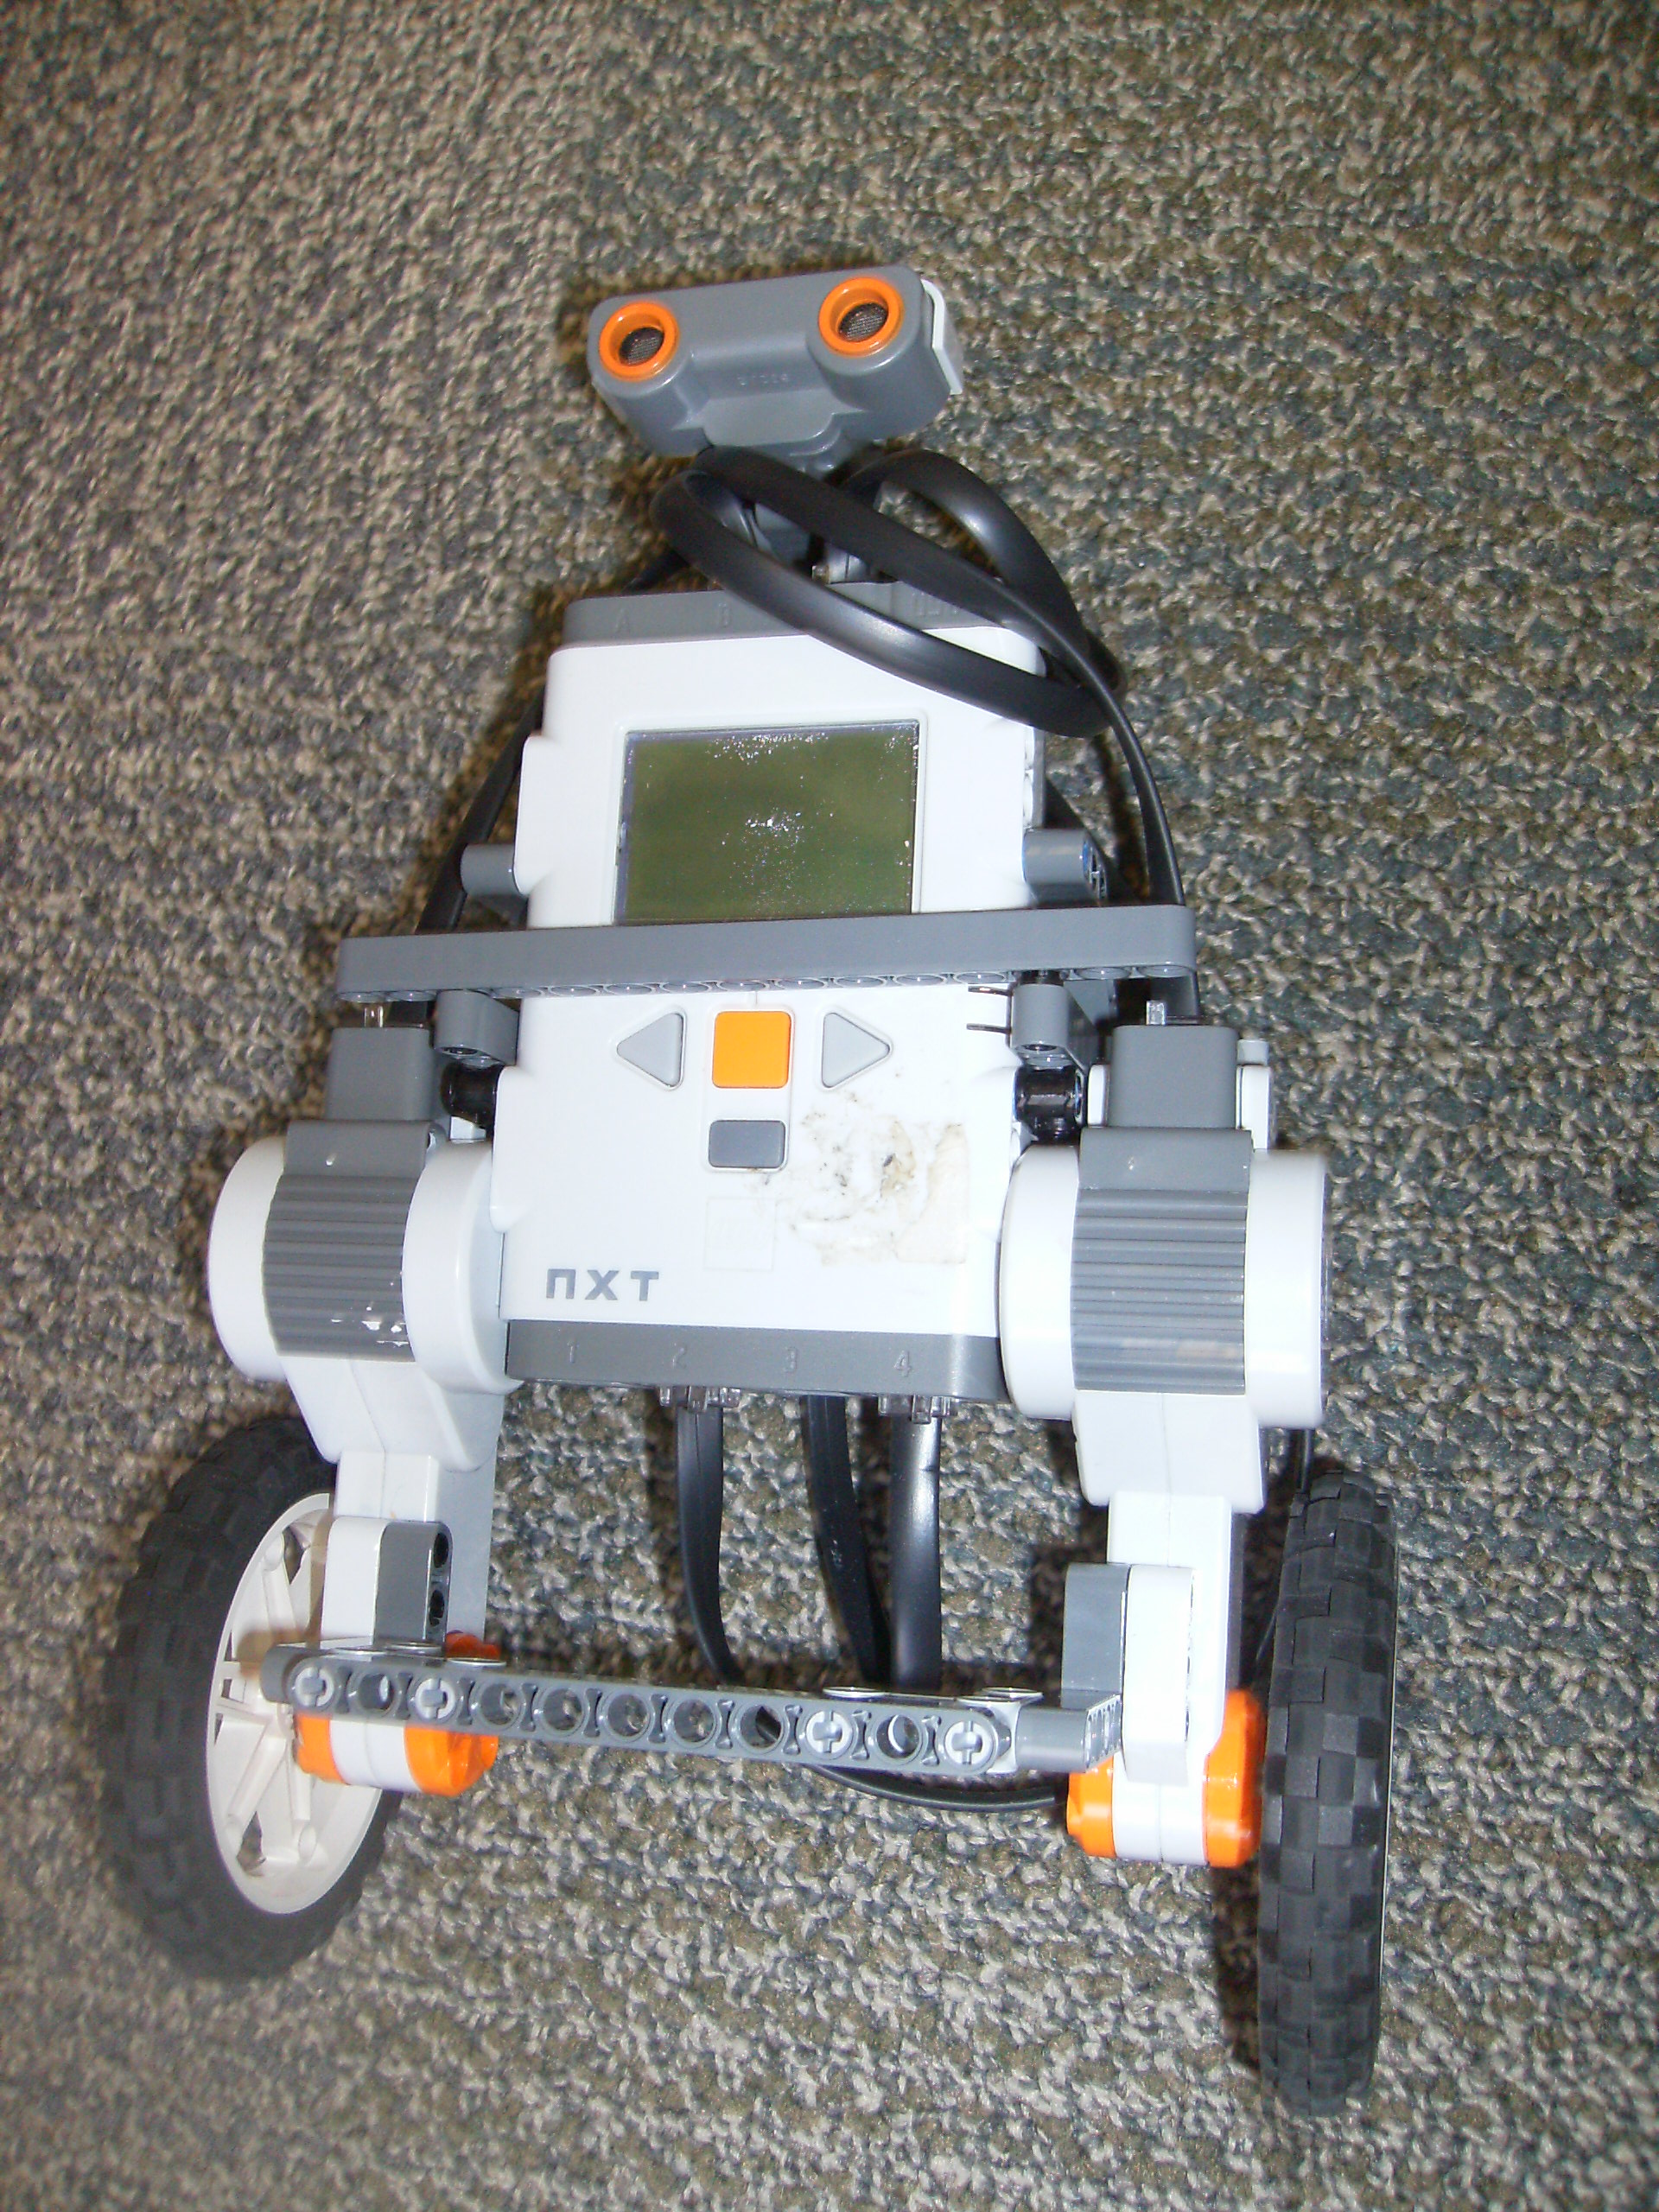
\includegraphics[scale=0.09]{fig/NXT-lego.JPG}
\end{figure}
\end{minipage}
\begin{minipage}{0.6\textwidth}
{\footnotesize Lego NXT self-balancing robot by\\ Medelen8/CC-BY-SA-3.0}
\begin{itemize}
\item \textcol{Sampled data Networked Control System}: Controller input to Plant sampled at discrete time instants.
\item Input from controller has \textcol{saturation} on {\color{violet} 2 controller inputs}: \textcol{Hybrid behavior}.
\end{itemize}
\end{minipage}

%% \begin{block}{}
%% $
%% \lt[\begin{array}{cc}\trj{x}{t+1} &
%%     \trj{y}{t+1}\end{array}\rt]^T=F_1\trj{x}{t}+F_2sat\lt(\trj{y}{t}\rt)+F_3\trj{u}{t}$\\
%% \textcol{Saturated}: $sat\lt(y_i\rt) = max\lt(-\delta
%% d_p,min\lt(y_i,\delta d_p\rt)\rt),~\forall i\in\{1,2\}$, where $\delta=100$
%% and $d_p=0.0807$. \textcol{Unsaturated}: $sat\lt(y_i\rt) = y_i$
%% \end{block}
\end{frame}


\begin{frame}{Verification challege: NXT-Lego Robot model}
\begin{alertblock}{Task}
Find/Verify bounds on \textcol{body pitch angle}.
\end{alertblock}
%
\eqncol{After transformation to decouple unbounded directions, we
obtained}\\
%
\begin{block}{Complexity}
\begin{itemize}
\item \eqncol{Saturated}: \textcol{9 dimensional, 1 location, 9 edges.}
\item \eqncol{Unsaturated}: \textcol{9 dimensional linear system.}
\end{itemize}
\end{block}
%
\end{frame}

\begin{frame}{Experimental settings}
%
\begin{itemize}
\item \eqncol{Primary template:}  (Complex) \textcol{Eigenvectors} of linear maps and their products,
 \textcol{Orthonormal
vectors} to guarding hyperplane normals.  For
the linear system, it consists of the eigenvectors of the linear map,
the \textcol{uncertain input set template} and its multiplication by the linear matrix
(related to affine map) and square of the linear matrix. 
\item \eqncol{SpaceEx settings:}  \textcol{Octagon template} and a
template with \textcol{$400$ uniformly sampled support vectors}.
\end{itemize}
%
\end{frame}


\begin{frame}{Results: NXT-Lego Robot model}
\center{{\eqncol{\small{\footnotesize UB: $>$1000, ~~NT: Not terminating in more than 180s, \newline
  n/a: Not applicable/not available, ~~ACZ: Augmented complex
  zonotope.}}}}
{\color{black}
\begin{minipage}{0.48\textwidth}
\begin{table}
\centering
\resizebox{0.5\textheight}{0.35\textwidth}{
\begin{tabular}{|l|c|c|c|}
\hline
\multicolumn{2}{|c|}{\multirow{2}{*}{Method}} &
\multirow{2}{*}{$\lt|\psi\rt|\leq$} & Comp.\\
\multicolumn{2}{|c|}{} & & time (s)\\
\hline
\multirow{4}{*}{SpaceEx} & octagon & \multirow{2}{*}{UB} & \multirow{2}{*}{NT}\\
& template & & \\
\cline{2-4}
& 400 support & \multirow{2}{*}{UB} & \multirow{2}{*}{NT}\\
& vectors & &\\
\hline
\multicolumn{2}{|c|}{\multirow{2}{*}{Suggested in~\cite{heinz2014benchmark}}} &
\multirow{2}{*}{$1.39$} & \multirow{2}{*}{n/a}\\
\multicolumn{2}{|c|}{} & &\\
\hline
\multicolumn{2}{|c|}{\multirow{2}{*}{ACZ invariant}} & \multirow{2}{*}{$1.29$} &
\multirow{2}{*}{$4$}\\
\multicolumn{2}{|c|}{} & & \\
\hline
\end{tabular}
}
\caption*{{\footnotesize Unsaturated robot model: results}}
\end{table}
\end{minipage}
\begin{minipage}{0.48\textwidth}
\begin{table}
\centering
\resizebox{0.5\textheight}{0.35\textwidth}{
\begin{tabular}{|l|c|c|c|}
\hline
\multicolumn{2}{|c|}{\multirow{2}{*}{Method}} &
\multirow{2}{*}{$\lt|\psi\rt|\leq$} & Comp.\\
\multicolumn{2}{|c|}{} & & time (s)\\
\hline
\multirow{4}{*}{SpaceEx} & octagon & \multirow{2}{*}{UB} &
\multirow{2}{*}{NT}\\
& template & & \\
\cline{2-4}
& 400 support & \multirow{2}{*}{UB} & \multirow{2}{*}{NT}\\
& vectors & & \\
\hline
\multicolumn{2}{|c|}{\multirow{2}{*}{Suggested in~\cite{heinz2014benchmark}}} &
$1.571-\epsilon:$ & \multirow{2}{*}{n/a}\\
\multicolumn{2}{|c|}{} & $\epsilon>0$ &\\
\hline
\multicolumn{2}{|c|}{\multirow{2}{*}{ACZ invariant}} & \multirow{2}{*}{$1.13$} &
\multirow{2}{*}{45}\\
\multicolumn{2}{|c|}{} & &\\
\hline
\end{tabular}
}
\caption*{{\footnotesize Saturated robot model: results}}
\end{table}
\end{minipage}
}
\vspace{-2em}
{\small
\begin{alertblock}{Remarks}
\begin{itemize}
\item Model has \textcol{complex eigenstructure}, some eigenvalues have \textcol{magnitude close to 1}.
\item Since \textcol{Complex Zonotope uses complex eigenstructure}, where as \textcol{Polytope (SpaceEx)} \eqncol{can not use complex eigenstructure}.
\end{itemize}
\end{alertblock}
}
\end{frame}

\begin{frame}{Example 2: Perturbed double integrator}
\begin{itemize}
\item Example from \textcol{Rakovic et. al.-CDC 2004}~\cite{rakovic2004computation}.
\item \textcol{Piecewise affine with 2 dimensional additive disturbance input}, \eqncol{Four different Affine
dynamics} in \eqncol{Four different polytopic regions} of space.
\item Model complexity: \textcol{2 dimensions, 4 locations and 12 edges.}
\end{itemize}
\begin{alertblock}{Challenge}
\begin{enumerate}
\item Verify \textcol{smallest (possible) bounds} on the \textcol{two state space co-ordinates}.
\item Compute a \textcol{large set} of \textcol{safe initial conditions}.
\end{enumerate}
\end{alertblock}
\pause
\begin{exampleblock}{Experimental settings}
\begin{itemize}
\item  {\bf Primary template}: \textcol{Complex eigenvectors} of all linear matrices of the \textcol{affine maps and
their binary products}. 
\item  {\bf SpaceEx tool}: \eqncol{Two
different templates}: \textcol{Octagon} template and a template with \textcol{100
uniformly sampled support vectors}.
\end{itemize}
\end{exampleblock}
\end{frame}

\begin{frame}{Experimental results: PDI}
\begin{table}
\begin{minipage}{\textwidth}
\center
\caption*{Small invariant computation}
{\small
\begin{tabular}{|l|c|c|c|c|}
\hline
\multicolumn{2}{|c|}{\multirow{2}{*}{Method}} &
\multirow{2}{*}{$\lt|x_1\rt|\leq$} & \multirow{2}{*}{$\lt|x_2\rt|\leq$} & Comp.\\
\multicolumn{2}{|c|}{} & & & time (s) \\
\hline
\multirow{4}{*}{SpaceEx} & octagon & \multirow{2}{*}{0.38} &
\multirow{2}{*}{0.43} & \multirow{2}{*}{1.7}\\
& template & & &\\
\cline{2-5}
& 100 support & \multirow{2}{*}{0.38} & \multirow{2}{*}{0.43} & \multirow{2}{*}{23.6}\\
& vectors & & &\\
\hline
\multicolumn{2}{|c|}{\multirow{2}{*}{ACZ invariant}} &
\multirow{2}{*}{0.38} & \multirow{2}{*}{0.36} & 
\multirow{2}{*}{5.1}\\
\multicolumn{2}{|c|}{} & & &\\
\hline
\end{tabular}
}
\end{minipage}
\hspace{4em}
\begin{minipage}{\textwidth}
\center
{\small
\caption*{Large invariant computation}
\begin{tabular}{|c|c|}
\hline
\multirow{2}{*}{Method} & Comp.\\
& time (s)\\
\hline
\multirow{2}{*}{MPT tool~\cite{rakovic2004computation}} & \multirow{2}{*}{107}\\
& \\
\hline
\multirow{2}{*}{ACZ} & \multirow{2}{*}{12}\\
& \\
\hline
\end{tabular}
}
\end{minipage}
\end{table}
\end{frame}

\begin{frame}{Example 3: Networked vehicle platoon}
\begin{figure}
\caption*{\small Benchmark {\color{blue}  2014 ARCH Workshop}: \eqncol{Makhlouf and Kowalewski~\cite{makhlouf2014networked}}}
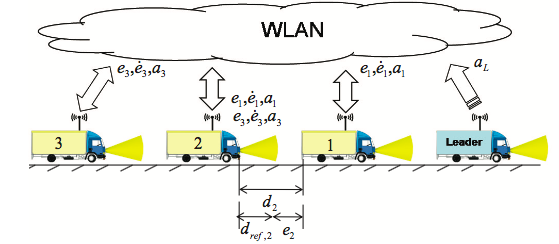
\includegraphics[scale=0.4]{fig/VehiclePlatoon.png}\\
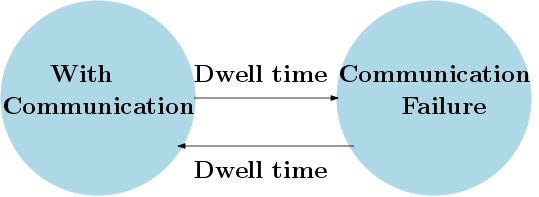
\includegraphics[scale=0.4]{fig/networked-platoon-model.png}
\end{figure}
\end{frame}

\begin{frame}{Verification challenge: Networked platoon}
\begin{alertblock}{Task}
\begin{itemize}
\item Find \textcol{minimum (possible) reference distances between vehicles} such that \eqncol{vehicles do not collide}.
\item Equivalent to finding \textcol{ upper bounds on $-e_1, -e_2$ and $-e_3$}.
\end{itemize}
\end{alertblock}
%
\begin{exampleblock}{Two cases}
\begin{enumerate}
\item \textcol{Slow switching}: \eqncol{Minimum dwell time 20 s}. {\color{violet} 9 dimensional, 2 locations, 4 edges}.
\item \textcol{Fast switching}: \eqncol{Integer dwell times}. {\color{violet} 9 dimensional, 2 locations, 2 edges}.
\end{enumerate}
\end{exampleblock}
\end{frame}

\begin{frame}{Expermimental results: Networked Platoon}
\begin{table}
\resizebox{1.1\textwidth}{!}{\hspace{-3em}
\begin{tabular}{|l|c|c|c|c|c|c|c|c|c|}
\hline
\multicolumn{2}{|c|}{\multirow{4}{*}{Method}} & \multicolumn{4}{|c|}{\multirow{2}{*}{Slow switching}} & \multicolumn{4}{|c|}{\multirow{2}{*}{Fast switching}}\\
\multicolumn{2}{|c|}{} & \multicolumn{4}{|c|}{} & \multicolumn{4}{|c|}{} \\
\cline{3-10}
\multicolumn{2}{|c|}{} & \multirow{2}{*}{$-e_1\leq$} & \multirow{2}{*}{$-e_2\leq$} & \multirow{2}{*}{$-e_3\leq$} & Comp. & \multirow{2}{*}{$-e_1\leq$} & \multirow{2}{*}{$-e_2\leq$} & \multirow{2}{*}{$-e_3\leq$} & Comp.\\
\multicolumn{2}{|c|}{} & & & & time (s) & & & & time (s)\\
\hline
\multirow{4}{*}{SpaceEx} & octagon & \multirow{2}{*}{28} &
\multirow{2}{*}{27} & \multirow{2}{*}{10} &
\multirow{2}{*}{NT} & \multirow{2}{*}{UB} &
\multirow{2}{*}{UB} & \multirow{2}{*}{UB} &
\multirow{2}{*}{NT}\\
& template & & & & & & & &\\
\cline{2-10}
& 100 support & \multirow{2}{*}{28} & \multirow{2}{*}{25} &
\multirow{2}{*}{13} & \multirow{2}{*}{1.3} & \multirow{2}{*}{UB} & \multirow{2}{*}{UB} &
\multirow{2}{*}{UB} & \multirow{2}{*}{NT}\\
& vectors & & & & & & & &\\
\hline
\multicolumn{2}{|c|}{\multirow{2}{*}{Real zonotope~\cite{makhlouf2014networked}}} &
\multirow{2}{*}{25} & \multirow{2}{*}{25} & \multirow{2}{*}{10}
 & \multirow{2}{*}{n/a} & \multirow{2}{*}{n/a} & \multirow{2}{*}{n/a} & \multirow{2}{*}{n/a}
 & \multirow{2}{*}{n/a}\\
\multicolumn{2}{|c|}{} & & & & & & & &\\
\hline
\multicolumn{2}{|c|}{\multirow{2}{*}{ACZ invariant}} &
\multirow{2}{*}{28} & \multirow{2}{*}{26} &
\multirow{2}{*}{12} & \multirow{2}{*}{12} &
\multirow{2}{*}{46} & \multirow{2}{*}{54} &
\multirow{2}{*}{57} & \multirow{2}{*}{12.6}\\
\multicolumn{2}{|c|}{} & & & & & & & &\\
\hline
\end{tabular}
}
%% \caption*{{\footnotesize UB: $>$1000, ~~NT: Not terminating in more than 180s, \newline
%%   n/a: Not applicable/not available, ~~ACZ: Augmented complex
%%   zonotope.
%% }}
{\small
\begin{alertblock}{Remarks}
\begin{itemize}
\item {\bf Slow switching model} is \textcol{more stable} than {\bf fast switching model}.
\item Since {\bf complex zonotope} used \textcol{eigenstructue}, it could also \textcol{compute invariant} for the \textcol{less stable: fast switching} model, while  {\bf Polytope (SpaceEx)} \eqncol{could not}.
\end{itemize}
\end{alertblock}
}
\end{table}
\end{frame}

\begin{frame}{Contributions}
\begin{enumerate}
\item Extend {\color{blue} real zonotopes to complex zonotopes} so as to capture
{\color{blue} contraction along complex eigenvectors}.
\item Derive {\color{blue} convex program} {\color{purple}(executed only
once)} to verify safety.  {\color{blue} Avoids ambiguity in
over-approximation} in safety verification.
\end{enumerate}
\end{frame}

\begin{frame}{References}

\begin{thebibliography}{1}

\bibitem{adimoolam2017augmented}
Arvind Adimoolam and Thao Dang.
\newblock Augmented complex zonotopes for computing invariants of affine hybrid
  systems.
\newblock In {\em International Conference on Formal Modeling and Analysis of
  Timed Systems}, pages 97--115. Springer, 2017.

\bibitem{girard2005reachability}
Antoine Girard.
\newblock Reachability of uncertain linear systems using zonotopes.
\newblock In {\em HSCC}, volume~5, pages 291--305. Springer, 2005.

\end{thebibliography}


\begin{itemize}
\item Template Complex Zonotope based Stability Verification - {\it Arvind
Adimoolam and Thao Dang}. \url{https://sites.google.com/site/arvind23adi/research/complex-zonotope}
\end{itemize}
\end{frame}


\begin{frame}{}
\center
{\Huge {\color{blue} Thank you!}}
\end{frame}













\bibliographystyle{plain}
\bibliography{ref}



\end{document}

